\documentclass{resume} % Use the custom resume.cls style



\usepackage[square,sort,comma,numbers]{natbib} % refer to https://tex.stackexchange.com/questions/54480/package-natbib-error-bibliography-not-compatible-with-author-year-citations to resolve the error...
\usepackage{bibentry}
\usepackage{xeCJK}
\usepackage{multicol}  % 提供多栏环境
\usepackage{graphicx} % For including images
\usepackage{amsmath,amsfonts}
\usepackage{bbm, bm}
 
\newcommand{\trianglebullet}{$\mbox{\ensuremath{\rhd}}$}


\usepackage[left=0.4 in,top=0.4in,right=0.4 in,bottom=0.4in]{geometry} % Document margins
\newcommand{\tab}[1]{\hspace{.2667\textwidth}\rlap{#1}} 
\newcommand{\itab}[1]{\hspace{0em}\rlap{#1}}
\name{苏隽岩} % Your name
% You can merge both of these into a single line, if you do not have a website.
%\address{+1(123) 456-7890 \\ San Francisco, CA} 
\address{个人主页: \href{https://sujunyan.github.io}{sujunyan.github.io}}
\address{电邮: \href{mailto:junyan.su@my.cityu.edu.hk}{junyan.su@my.cityu.edu.hk} 
    \\ 手机: 15002127975
    }

% 项目经历标题格式定义(可复用)
\newcommand{\projectheader}[3]{%
  % \vspace{0.5em} % 标题与内容的间距
  \begin{tabular*}{\linewidth}{@{}l@{\extracolsep{\fill}}l@{\extracolsep{\fill}}r@{}}
% \begin{tabular*}{\linewidth}{@{}>{\bfseries}l@{\extracolsep{\fill}}>{\bfseries}l@{\extracolsep{\fill}}>{\bfseries}l@{}}
    \textbf{#1} & \textbf{#2} & \textbf{#3} \\
  \end{tabular*}%
  \vspace{-0.5em} % 标题与内容的间距
}



% \\ \href{https://linkedin.com/in/linkedinURL}{linkedin.com/in/linkedinURL}   %


% \usepackage[backend=bibtex]{biblatex}
% \addbibresource{\jobname.bib}
\begin{document}

\bibliographystyle{abbrv1}
\nobibliography{../../../_bibliography/underreview, ../../../_bibliography/papers}
% \nobibliography{../../../_bibliography/papers.bib}

%----------------------------------------------------------------------------------------
%----------------------------------------------------------------------------------------
%	EDUCATION SECTION
%----------------------------------------------------------------------------------------

\begin{rSection}{研究方向}
    % 智慧交通系统,主要从控制与优化的角度进行研究。同时,我也对能源系统的计算方法有广泛的兴趣。
    我的研究聚焦于智慧交通系统的控制与优化,通过设计节能导航算法(如路径-速度联合优化)和MPC控制方法, 设计解决高能耗、高排放的交通问题。
    % 同时探索优化理论在能源系统(如多库存管理)中的跨领域应用,推动可持续发展。
\end{rSection}

\begin{rSection}{教育经历}

% \begin{itemize}
    \textbf{香港城市大学}  \hfill {2020.10-2025.10} 
    \\ 数据科学博士 | 指导老师:陈名华教授 
    \begin{itemize}
        \item 毕业论文:重型卡车及时运输中的排放及碳足迹的优化。
    \end{itemize}
    % \\ \trianglebullet 

    \textbf{圣路易斯华盛顿大学}  \hfill {2019.09}
    \\ 系统科学与数学博士 |(拟入学、因签证原因更换学校) 

    \textbf{上海科技大学}  \hfill {2015.09-2019.06} 
    \\ 计算机科学与技术学士 | 指导老师:Boris Houska教授、姜育宁博士 
    \\ GPA: 3.84/4.0, 专业排名: 3/95
    \begin{itemize}
        \item 核心课程:数据结构(A+)、计算机体系结构(A)、信号与系统(A)、控制原理(A+)、操作系统(A-)、离散数学(A)、算法基础(A)。
        \item 毕业设计:ALADIN 算法在分布式机器学习中的应用。
    \end{itemize}
    % \\ \trianglebullet 
    % \\ \trianglebullet

    % \\ 毕业论文题目:\textit{Optimizing Carbon Footprint in Long-Haul Heavy-Duty E-Truck Transportation}。

% \end{itemize}

\end{rSection}







% My research interests are intelligent transportation systems, from the perspective of control and optimization. I also have broad interests in computing methods for energy systems.

\def\FormatName#1{%
    \def\myname{Junyan Su}%
    \edef\name{#1}%
    \ifx\name\myname
      \underline{#1}%
    \else
       #1%
    \fi
}

\begin{rSection}{项目经历}
    % {主导开发了\href{https://www.e2pilots.com/}{\textcolor{blue}{E2Pilot}}}, 一款专为重型卡车长途运输设计的节能导航系统:
    \projectheader{2022.01-至今}{\href{https://www.e2pilots.com/}{\textcolor{black}{E2Pilot}}: 重卡长途节能导航系统}{技术负责人}

    \begin{minipage}[h]{0.65\textwidth} % 左边文字部分,占60%宽度
        % \trianglebullet 项目包括网页端和移动端应用。用户只需输入起点、目的地及取送货时间窗,系统即可规划出最经济的路线和车速。% 通过实时车速指引,确保用户能够在准时送达的同时实现燃油成本节约。
        % \trianglebullet 项目已成功完成首次实车路测,相关成果已发表多篇论文(包括一篇子刊 \textcolor{blue}{Nature Communications})。
        % \trianglebullet 项目已获得HK Tech 300 \& HKTSP种子基金支持。
        % \trianglebullet 使用的技术栈包括 Julia、JavaScript、Swift、JuMP.jl、Gurobi等。项目链接:\href{https://www.e2pilots.com/}{https://www.e2pilots.com}。
         \begin{itemize}
            \item 项目包括网页端和移动端应用。用户只需输入起点、目的地及取送货时间窗,系统即可规划出最经济的路线和车速。% 通过实时车速指引,确保用户能够在准时送达的同时实现燃油成本节约。
            \item 项目已成功完成首次实车路测,相关成果已发表多篇论文(包括一篇子刊 \textcolor{blue}{Nature Communications})。
            \item 项目已获得HK Tech 300 \& HKTSP种子基金支持。
            \item 使用的技术栈包括 Julia、JavaScript、Swift、JuMP.jl、Gurobi等。项目链接:\href{https://www.e2pilots.com/}{https://www.e2pilots.com}。
        \end{itemize}
    \end{minipage}%
    \hfill % 在左右两部分之间添加间距
    \begin{minipage}[h]{0.35\textwidth} % 右边图片部分,占35%宽度
        \centering
        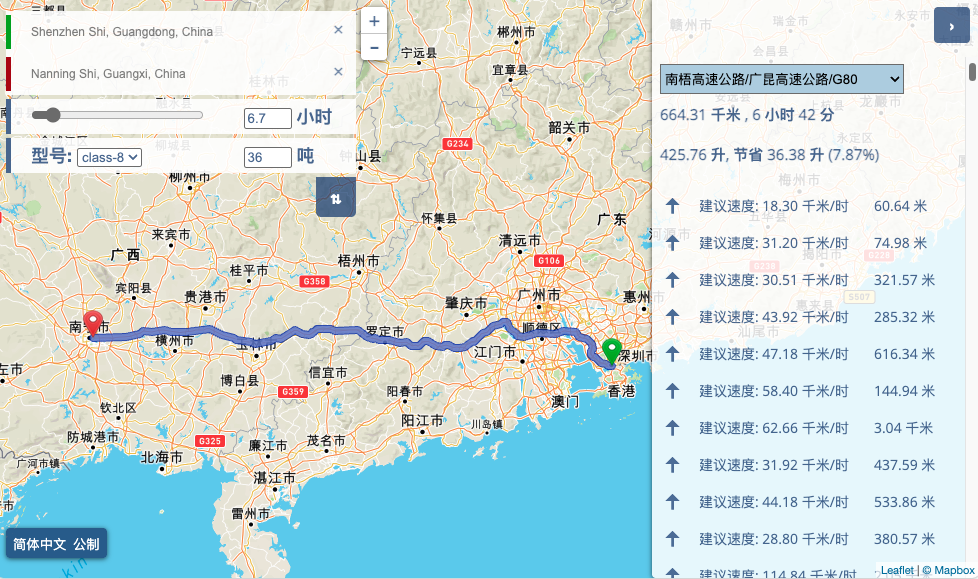
\includegraphics[width=.80\textwidth]{e2pilot-web.png} % 替换为你的图片路径
        % \captionof{figure}{E2Pilot 系统界面} % 可选的图片标题
    \end{minipage}


    % \newpage
    \vspace{3mm}
    % 主导开发了\href{https://github.com/sujunyan/ParExMPC}{\textcolor{blue}{ParExMPC}}:
    \projectheader{2020.01-2024.12}{ParExMPC: 轻量模型预测控制(MPC)设计工具箱}{技术负责人}
    \begin{itemize}
        % \item ParExMPC 是一款模型预测控制(MPC)设计工具箱。
        \item 给定一个非线性系统模型和一个优化目标,用户可通过工具箱的MATLAB界面生成一个 轻量MPC 控制器。相关成果已发表论文。
        \item 工具箱可生成C代码。生成的代码可部署在最低内存2kb嵌入式设备上。
        \item 使用技术栈包括MATLAB、C。 项目链接:\href{https://github.com/sujunyan/ParExMPC/wiki}{https://github.com/sujunyan/ParExMPC/wiki}。
        % \item 提供基于 MATLAB 的用户界面和定制的 C 代码求解器。
    \end{itemize}

    \vspace{3mm}
    \projectheader{2023.08-2023.12}{美团低空经济挑战赛}{调度部分技术开发}
    \begin{itemize}
        \item 美团低空经济挑战赛旨在解决多机路径规划与调度问题。赛方提供仿真平台,由选手开发算法调度完成订单。
        \item 主要负责设计和实现无人机调度算法。根据当前订单需求,优化调度多架无人机前往各地完成订单/更换电池。
        \item 主要技术栈为C++、Google OR-Tools。取得2023年性能赛第二名。
    \end{itemize}


    % 主导参加\href{https://www.robomaster.com/zh-CN}{\textcolor{blue}{RoboMaster 2018 机甲大师赛}}(电控部分):
    % \vspace{3mm}
    % \projectheader{2017.09-2018.05}{RoboMaster 机甲大师赛}{电控组负责人}
    % \begin{itemize}
    %     \item 在团队中全面负责电控系统,涵盖嵌入式软件、硬件及整机电子架构。基于官方推荐的 STM32F4xx 开发版,引入 FreeRTOS 多线程框架,自底向上实现驱动层、控制层与指令级功能。
    %     \item 使用技术栈:电路设计、嵌入式 C、STM32、FreeRTOS。
    % \end{itemize}

    % \item 项目链接: \href{https://github.com/sujunyan/ShanghaiTech\_Robomasters2018}{https://github.com/sujunyan/ShanghaiTech\_Robomasters2018}
    % \textbf{Main developer} of the \href{https://www.e2pilots.com/}{\textcolor{blue}{E2Pilot}}, a navigation platform for energy-efficient long-haul timely truck transportation. \\
    % \textbf{Main developer} of the \href{https://github.com/sujunyan/ParExMPC}{\textcolor{blue}{ParExMPC}}, an open-source toolbox for real-time close-to-optimal Model Predictive Control (MPC) design providing MATLAB-based user interface and tailored C-code solver. \\
    % \textbf{Main contributor} of the simulation for ALL the publication I co-authored. \\
    % \textbf{Programming languages:} working knowledge of Julia, Python, C/C++, MATLAB.
\end{rSection}

\newpage
\begin{rSection}{访学交流经历}
     % \begin{itemize}
    \textbf{瑞典皇家理工学院}  \hfill {2024.05-2024.09}
    \\ 访问学生 | 指导老师:Karl H. Johansson教授
    \begin{itemize}
        \item 研究探索优化理论在无人机及卡车编队中的应用。
    \end{itemize}
    % \\ \trianglebullet 

    \textbf{卡耐基梅隆大学} \hfill {2018.06-2018.08} 
    \\ RISS机器人暑期项目访问学生 | 指导老师:Howie Choset教授
    \begin{itemize}
        \item 使用Verilog设计逻辑电路实现I2C协议,从多传感器获取数据并显著减少CPU干预时间。
    \end{itemize}
    % \\ \trianglebullet 
    \textbf{加州大学伯克利分校}  \hfill {2018.08-2019.05} 
    \\ 访问学生 | GPA: 3.95/4.0 
    \begin{itemize}
        \item 核心课程:机器人导论(A)、线性系统理论(A)、机电一体化(A)、编程语言与编译器(A-)、机器人控制与交互(A)、数值计算方法(A)。
    \end{itemize}
    % \\ \trianglebullet 
    % \end{itemize}
\end{rSection}


% \begin{rSection}{Working Papers}
%     \begin{enumerate}
%          \item \bibentry{su2025maximizing}.
%          \item \bibentry{lin2025optimal}.
%     \end{enumerate}
%          % \item \bibentry{su2025maximizing}.
% \end{rSection}

\begin{rSection}{奖项与荣誉}

    % \begin{multicols}{2} 
    \begin{itemize}
        \item 竞赛奖项: 2023年美团低空经济挑战赛第二名
        % \end{itemize}
        \item 学术奖项: 
        2023年香港城市大学杰出学术表现奖、2023年 ACM e-Energy 最佳论文奖
        \item 创业资助: 2022年 HK Tech 300 \& HKTSP 种子基金获得者
        \item 学生奖项与资助:
        2023年CDC学生旅行资助与研讨会支持、2019 年上海科技大学优秀毕业生
        % \begin{itemize}
        % \end{itemize}
        % \begin{itemize}
        % \end{itemize}
        % \begin{itemize}
        % \end{itemize}
        % \item 竞赛奖项: 
        % \begin{itemize}
        %     \item 2023年美团低空经济挑战赛第二名
        % \end{itemize}
        % \item 学术奖项: 
        % \begin{itemize}
        %     \item 2023年香港城市大学杰出学术表现奖
        %     \item 2023年 ACM e-Energy 最佳论文奖
        % \end{itemize}
        % \item 创业资助: 
        % \begin{itemize}
        %     \item 2022年 HK Tech 300 \& HKTSP 种子基金获得者
        % \end{itemize}
        % \item 学生奖项与资助:
        % \begin{itemize}
        %     \item 2023年CDC学生旅行资助与研讨会支持
        %     \item 2019 年上海科技大学优秀毕业生
        % \end{itemize}
        % \item 香港城市大学研究生学费奖学金, 2023
        % \item ACM e-Energy 最佳论文奖, 2023
        % \item 上海科技大学优秀毕业生, 2019
    \end{itemize}
    % \end{multicols}  % 双栏结束
    % \vspace{-5mm}
    % Second Place, Meituan UAV Competition, 2023. \\
    % CDC Student Travel Grant \& Workshop Support, 2023. \\
    % Research Tuition Scholarship, City University of Hong Kong, 2023. \\
    % Outstanding Academic Performance Award, City University of Hong Kong, 2023. \\
    % ACM e-Energy Best Paper Award, 2023. \\
    % HK Tech 300 \& HKTSP Seed Fund, 2022. \\
    % Outstanding Graduate, ShanghaiTech University, 2019. 
    % Outstanding Student, ShanghaiTech University, 2016,2017,2018.
\end{rSection}

% \newpage



% \newpage

% \begin{rSection}{Presentations}
%     \begin{itemize}
%         \item ``E2Pilot: A Navigation Platform for Energy-Efficient Timely Transportation of Long-Haul Heavy-Duty Trucks'', Prototypes for Humanity, Dubai, November 2024.
%         \item ``Minimizing Carbon Footprint for Timely E-Truck Transportation: Hardness and Approximation Algorithm'', 
%         CDC 2023, Singpore, December 2023.
%         \item ``Follow the Sun and Go with the Wind: Carbon Footprint Optimized Timely E-Truck Transportation'', ACM e-Energy 2023, Orlando, Florida, June 2023.
%     \end{itemize}
% \end{rSection}
\begin{rSection}{专利}
    \begin{itemize}
        \item M. Chen., \underline{J. Su}, and Q. Lin, ``Carbon Footprint Optimized Timely E-Truck Transportation", 14 Aug 2025, U.S. Patent No. US2025/0258006.
        % Carbon Footprint Optimized Timely E-Truck Transportation CHEN, M., SU, J. & LIN, Q., 8 Feb 2024, (Filed) Priority No. 18/436,350 Research output: Patents, Agreements and Assignments › RGC 51 - Patents (CityU)
    \end{itemize}
\end{rSection}
% \newpage

\begin{rSection}{期刊论文}
    % $^*:$ Co-primary author. 
    \begin{enumerate}
        % \item \bibentry{su2025optimizing}.
        \item \underline{Junyan Su}, Qiulin Lin, and Minghua Chen. Optimizing Carbon Footprint in Long-Haul Heavy-Duty E-Truck Transportation. \textcolor{blue}{\textit{Nature Communications}}, accepted for publication. 
        \item \bibentry{lin2025optimala}.
        \item \bibentry{jiang2025fast}.
        \item \bibentry{su2024minimizing}.
        \item \bibentry{jiang2020distributed}.
    \end{enumerate}
\end{rSection}

\begin{rSection}{会议论文}
    % \bibliographystyle{mybibstyle}
    %% Refer to the following link to highlight my own name.
    %% https://tex.stackexchange.com/questions/33330/make-one-authors-name-bold-every-time-it-shows-up-in-the-bibliography/33379#33379
    
    % \nobibliography{papers.bib}
    \begin{enumerate}
         \item \bibentry{lin2024competitive}.
         \item \bibentry{su2023minimize}.
         \item \bibentry{su2023follow}. \textcolor{blue}{Best Paper Award}.
    % \begin{enumerate}
    %     \item \bibentry{su2023follow} \textbf{(Best Paper Award)}
    %     \item \bibentry{jiang2020distributed}
    % \end{enumerate}
    % \textbf{Other Publication:}
        \item \bibentry{lin2022competitive}.
        % \item \bibentry{su2022e2pilot}.
        % \item \bibentry{su2021energy}.
        \item \bibentry{su2020distributed}.
        \item \bibentry{gao2020efficient}.
        % \item \bibentry{su2019interval}.
    \end{enumerate}
\end{rSection}

% \newpage
\begin{rSection}{其它课程项目}
    \begin{multicols}{2} 
    \begin{itemize}
        \item 最优800MHz 6位绝对值检测器 (Cadence)
        \item 用强化学习游玩吃豆人游戏 (Python、RL) 
        % \href{https://github.com/sujunyan/SDSC8006RL_project}{\textcolor{blue}{[链接]}}
        \item 斯坦福Pintos课程项目 (OS、C语言)
        \item 参与主导RoboMaster 电控部分 (STM32、C语言)
        \item 伯克利机器人课程项目(控制小车、机械臂)(ROS) % \newline
        \item ``别碰我''机器人 (电路/机械设计、Arduino)
        % \href{https://github.com/sujunyan/SDSC8006RL_project}{\textcolor{blue}{[链接]}}
        % \item 曾经使用过 ROS、Cadence、Verilog、JavaScript、Swift。
    \end{itemize}
    \end{multicols}  % 双栏结束
    \vspace{-5mm}
\end{rSection}

\begin{rSection}{专业技能}
    \begin{itemize}
        \item 参与了共同署名的\textcolor{blue}{所有论文}的仿真工作
        \item 编程语言:Julia、Python、C/C++、MATLAB、JavaScript、Swift
        \item 机器人相关: ROS、STM32、Arduino、SolidWorks、RTOS、3D打印、PCB电路设计
        \item 优化运筹工具: JuMP.jl、Gurobi、Google OR-Tools
        \item 其它软件/工具: Cadence、Verilog、Git、Linux 开发环境、LaTeX
    \end{itemize} 
\end{rSection}



%----------------------------------------------------------------------------------------
% TECHINICAL STRENGTHS	
%----------------------------------------------------------------------------------------
% \begin{rSection}{SKILLS}
% \begin{tabular}{ @{} >{\bfseries}l @{\hspace{6ex}} l }
% Progamming Languages & Julia, Python, C/C++, MATLAB \\
% % Frameworks & React, Redux, Node.js, Express, Django, Mocha \\
% % Tools & Git, Docker, TravisCI, Kubernetes, AWS\\
% % Soft Skills & Time Management, Teamwork, Communication, Problem Solving, Leadership, Accountability
% \end{tabular}\\
% \end{rSection}


%----------------------------------------------------------------------------------------
% Projects
%----------------------------------------------------------------------------------------
%\begin{rSection}{PROJECTS}
%\vspace{-1.25em}
%\item \textbf{Project 1} {Language 1, Framework 1, Database, Language 2, Framework 2, DevOps Tooling} \hfill \href{www.github.com/GITHUBURL}{GitHub}
%\begin{itemize}
%    \itemsep -3pt {} 
%     \item Created a XYZ feature to accomplish ABC.
%     \item Retrieved data from XYZ to for ABC.
%    \item Implemented XYZ library for ABC.
%    \item Utilized XYZ that increased A by B\%.
% \end{itemize}
%\item \textbf{Project 2} {Language 1, Framework 1, Database, Language 2, Framework 2, DevOps Tooling} \hfill \href{www.github.com/GITHUBURL}{GitHub}
%\begin{itemize}
%    \itemsep -3pt {} 
%     \item Created a XYZ feature to accomplish ABC.
%     \item Retrieved data from XYZ to for ABC.
%    \item Implemented XYZ library for ABC.
%    \item Utilized XYZ that increased A by B\%.
% \end{itemize}
%\item \textbf{Project 3} {Language 1, Framework 1, Database, Language 2, Framework 2, DevOps Tooling} \hfill \href{www.github.com/GITHUBURL}{GitHub}
%\begin{itemize}
%    \itemsep -3pt {} 
%     \item Created a XYZ feature to accomplish ABC.
%     \item Retrieved data from XYZ to for ABC.
%    \item Implemented XYZ library for ABC.
%    \item Utilized XYZ that increased A by B\%.
% \end{itemize}
%\end{rSection} 

%----------------------------------------------------------------------------------------
% \begin{rSection}{Extra-Curricular Activities} 
% \begin{itemize}
%     \item 	Sample bullet point.
%     \item	Sample bullet point.
% \end{itemize}
% 
% 
% \end{rSection}

%------------------------
% Use this more detailed section if you have Relevant work experience
% keep your resume to 1 page, if you need to remove a project to display relevant experience
% that is okay
% ----------------------------
% \begin{rSection}{EXPERIENCE}

% \textbf{Role Name} \hfill Jan 2017 - Jan 2019\\
% Company Name \hfill \textit{San Francisco, CA}
%  \begin{itemize}
%     \itemsep -3pt {} 
%      \item Achieved X\% growth for XYZ using A, B, and C skills.
%      \item Led XYZ which led to X\% of improvement in ABC
%     \item Developed XYZ that did A, B, and C using X, Y, and Z. 
%  \end{itemize}
 
% \textbf{Role Name} \hfill Jan 2017 - Jan 2019\\
% Company Name \hfill \textit{San Francisco, CA}
%  \begin{itemize}
%     \itemsep -3pt {} 
%      \item Achieved X\% growth for XYZ using A, B, and C skills.
%      \item Led XYZ which led to X\% of improvement in ABC
%     \item Developed XYZ that did A, B, and C using X, Y, and Z. 
%  \end{itemize}

% \end{rSection} 

%\begin{rSection}{Work History}
%\vspace{-1.25em}
%\item \textbf{Job Title} {Company} \hfill Month Year - Month Year
%\item \textbf{Job Title} {Company} \hfill Month Year - Month Year
%\item \textbf{Job Title} {Company} \hfill Month Year - Month Year
%\end{rSection} 

%----------------------------------------------------------------------------------------

\end{document}
